\chapter{Integration: The Fundamental Theorem of Calculus}

\section{From Differentiation to Integration}

\begin{intuition}
Differentiation asks: ``What is the rate of change?''

Integration asks two related questions:
\begin{enumerate}
    \item \textbf{Antiderivative problem}: What function has $f$ as its derivative?
    \item \textbf{Area problem}: What is the area under the curve $y = f(x)$?
\end{enumerate}

\textbf{The miracle}: These two problems have the \textit{same answer}.

The \textbf{Fundamental Theorem of Calculus} connects them:
\[\text{Area under } f \text{ from } a \text{ to } b = F(b) - F(a), \quad \text{where } F' = f\]

This chapter makes this connection rigorous.
\end{intuition}

\begin{historicalnote}
\textbf{Ancient Origins (300 BCE - 1600 CE)}

\textbf{Archimedes (c. 250 BCE)}:
\begin{itemize}
    \item Computed areas using \textbf{method of exhaustion}
    \item Found area of parabolic segment: $\frac{4}{3} \times \text{triangle}$
    \item Computed $\pi$ by exhausting circle with polygons
    \item Method: Inscribe and circumscribe, then squeeze
\end{itemize}

\textbf{The Dark Ages (500-1400 CE)}: Greek works preserved in Arabic translations

\textbf{Early Modern (1400-1650)}:
\begin{itemize}
    \item \textbf{Cavalieri (1635)}: ``Indivisibles''---areas as infinite sums of lines
    \item \textbf{Fermat (1636)}: Found areas under $y = x^n$ by summing rectangles
    \item \textbf{Wallis (1656)}: Extended to rational exponents
\end{itemize}

\textbf{The Breakthrough (1665-1675)}

\textbf{Newton (1665-1666)} (unpublished until 1704):
\begin{itemize}
    \item Discovered: Antiderivatives compute areas
    \item \textit{``Integration is the inverse of differentiation''}
    \item Used for orbits, optics, gravitation
\end{itemize}

\textbf{Leibniz (1673-1675)}:
\begin{itemize}
    \item Independent discovery of Fundamental Theorem
    \item Invented notation: $\int$ (elongated S for ``sum''), $dx$ (infinitesimal)
    \item $\int f(x) \, dx$ read as ``sum of $f(x)$ times infinitesimal $dx$''
    \item His notation won: we still use $\int$ and $dx$ today
\end{itemize}

\textbf{18th Century (1700-1800)}: Euler, Lagrange, Laplace---powerful techniques, no rigor

\textbf{Rigorization (1800-1900)}

\textbf{Cauchy (1823)}:
\begin{itemize}
    \item First rigorous definition of integral as limit of sums
    \item Proved Fundamental Theorem using limits
\end{itemize}

\textbf{Riemann (1854)}:
\begin{itemize}
    \item Generalized Cauchy's approach
    \item \textbf{Riemann integral}: $\int_a^b f = \lim \sum f(x_i^*) \Delta x_i$
    \item Characterized integrable functions (continuous except at finitely many points)
\end{itemize}

\textbf{20th Century}: Lebesgue (1902) invented more powerful integral for measure theory. But Riemann's integral suffices for calculus.

\textbf{Modern view}: Integration is the inverse of differentiation, and also computes signed areas.
\end{historicalnote}

\section{The Riemann Integral: Definition}

\begin{definition}[Partition]
A \textbf{partition} of $[a, b]$ is a finite sequence:
\[P = \{x_0, x_1, \ldots, x_n\} \quad \text{where} \quad a = x_0 < x_1 < \cdots < x_n = b\]

The \textbf{mesh} or \textbf{norm} of $P$ is:
\[\|P\| = \max_{1 \leq i \leq n} (x_i - x_{i-1})\]
(the width of the largest subinterval).
\end{definition}

\begin{definition}[Riemann Sum]
Let $f: [a, b] \to \mathbb{R}$ be bounded, and let $P = \{x_0, \ldots, x_n\}$ be a partition.

Choose \textbf{sample points} $x_i^* \in [x_{i-1}, x_i]$ for each $i$.

The \textbf{Riemann sum} is:
\[S(f, P, \{x_i^*\}) = \sum_{i=1}^n f(x_i^*)(x_i - x_{i-1}) = \sum_{i=1}^n f(x_i^*) \Delta x_i\]

\textbf{Geometric interpretation}: Sum of signed areas of rectangles.
\end{definition}

\begin{center}
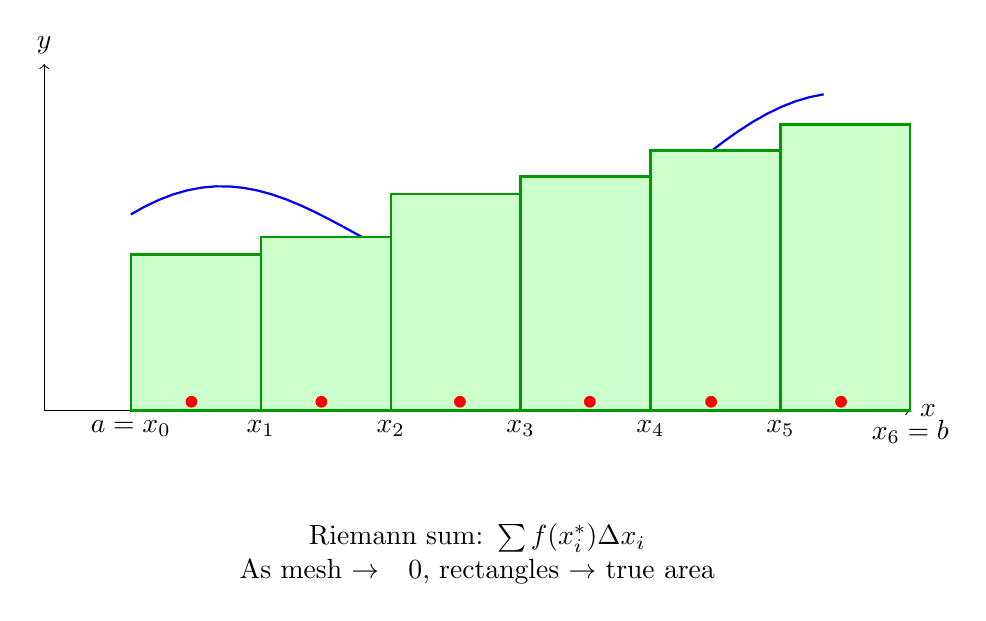
\begin{tikzpicture}[scale=1.1]
    \draw[->] (0, 0) -- (10, 0) node[right] {$x$};
    \draw[->] (0, 0) -- (0, 4) node[above] {$y$};
    
    % Function curve
    \draw[thick, blue, domain=1:9, samples=50] plot (\x, {1.5 + 0.8*sin(50*\x) + 0.15*\x});
    
    % Partition rectangles
    \foreach \x/\h in {1/1.8, 2.5/2.0, 4/2.5, 5.5/2.7, 7/3.0, 8.5/3.3} {
        \draw[thick, green!60!black, fill=green!20] (\x, 0) rectangle ++(1.5, \h);
    }
    
    % Points
    \node[below] at (1, 0) {$a=x_0$};
    \node[below] at (2.5, 0) {$x_1$};
    \node[below] at (4, 0) {$x_2$};
    \node[below] at (5.5, 0) {$x_3$};
    \node[below] at (7, 0) {$x_4$};
    \node[below] at (8.5, 0) {$x_5$};
    \node[below] at (10, 0) {$x_6=b$};
    
    % Sample points
    \foreach \x in {1.7, 3.2, 4.8, 6.3, 7.7, 9.2} {
        \node[circle, fill=red, inner sep=1.5pt] at (\x, 0.1) {};
    }
    
    \node[below, text width=10cm, align=center] at (5, -1.2) {
        Riemann sum: $\sum f(x_i^*) \Delta x_i$ \\
        As mesh $\to 0$, rectangles $\to$ true area
    };
\end{tikzpicture}
\end{center}

\begin{definition}[Riemann Integrability]
A function $f: [a, b] \to \mathbb{R}$ is \textbf{Riemann integrable} if there exists $L \in \mathbb{R}$ such that:

For every $\epsilon > 0$, there exists $\delta > 0$ such that for \textit{any} partition $P$ with $\|P\| < \delta$ and \textit{any} choice of sample points $\{x_i^*\}$:
\[|S(f, P, \{x_i^*\}) - L| < \epsilon\]

We write $L = \int_a^b f(x) \, dx$ and call this the \textbf{Riemann integral} of $f$ over $[a, b]$.

\textbf{In words}: All Riemann sums converge to the same limit as mesh $\to 0$.
\end{definition}

\begin{remark}[Alternative Approach: Darboux Sums]\index{Darboux sums}
The Riemann integral as defined above uses \textbf{tagged partitions} (partitions with chosen sample points). This is intuitive but technically cumbersome for proofs.

An equivalent definition uses \textbf{Darboux sums} (upper and lower sums):
\begin{align*}
U(f, P) &= \sum_{i=1}^n \sup_{x \in [x_{i-1}, x_i]} f(x) \cdot (x_i - x_{i-1}) \quad \text{(Upper sum)} \\
L(f, P) &= \sum_{i=1}^n \inf_{x \in [x_{i-1}, x_i]} f(x) \cdot (x_i - x_{i-1}) \quad \text{(Lower sum)}
\end{align*}

A function is Riemann integrable if and only if:
\[\sup_P L(f, P) = \inf_P U(f, P)\]

\textbf{Advantage}: No need to consider all possible sample point choices---just supremum and infimum over each subinterval. Many theorems (especially integrability criteria) have cleaner proofs using Darboux sums.

For this text, we use the tagged partition approach for its intuitive connection to approximating areas, but readers should be aware that the Darboux formulation is often preferred for technical work.
\end{remark}

\begin{keyidea}
\textbf{Three key ideas}:
\begin{enumerate}
    \item The integral is a \textbf{limit} (like derivatives)
    \item The limit must be \textbf{independent} of choice of partition and sample points
    \item Not all functions are integrable (e.g., Dirichlet's function: $f(x) = 1$ if $x \in \mathbb{Q}$, $f(x) = 0$ if $x \notin \mathbb{Q}$)
\end{enumerate}
\end{keyidea}

\begin{theorem}[Continuous Functions are Integrable]
If $f: [a, b] \to \mathbb{R}$ is continuous, then $f$ is Riemann integrable.
\end{theorem}

\begin{proof}[Proof Sketch]
Since $f$ is continuous on the compact interval $[a, b]$, by uniform continuity theorem (Chapter 11), $f$ is uniformly continuous.

Given $\epsilon > 0$, choose $\delta > 0$ such that:
\[|x - y| < \delta \implies |f(x) - f(y)| < \frac{\epsilon}{b - a}\]

For any partition $P$ with $\|P\| < \delta$, on each subinterval $[x_{i-1}, x_i]$, the variation of $f$ is at most $\frac{\epsilon}{b-a}$.

Therefore, for any two choices of sample points, the Riemann sums differ by at most:
\[\sum_{i=1}^n \frac{\epsilon}{b-a} (x_i - x_{i-1}) = \frac{\epsilon}{b-a} \cdot (b - a) = \epsilon\]

By Cauchy criterion (analogous to sequences), the Riemann sums converge. $\blacksquare$

(A complete proof requires more care with the Cauchy criterion for integrals.)
\end{proof}

\section{Properties of the Integral}

\begin{theorem}[Linearity of Integration]
If $f$ and $g$ are integrable on $[a, b]$, then:
\begin{enumerate}
    \item $\int_a^b [f(x) + g(x)] \, dx = \int_a^b f(x) \, dx + \int_a^b g(x) \, dx$
    \item $\int_a^b cf(x) \, dx = c \int_a^b f(x) \, dx$ for any $c \in \mathbb{R}$
\end{enumerate}
\end{theorem}

\begin{proof}
These follow directly from linearity of limits and sums:
\[\sum [f(x_i^*) + g(x_i^*)] \Delta x_i = \sum f(x_i^*) \Delta x_i + \sum g(x_i^*) \Delta x_i\]

Taking limits as $\|P\| \to 0$ gives the result. $\blacksquare$
\end{proof}

\begin{theorem}[Comparison Properties]
If $f$ and $g$ are integrable on $[a, b]$:
\begin{enumerate}
    \item If $f(x) \geq 0$ for all $x \in [a, b]$, then $\int_a^b f(x) \, dx \geq 0$
    \item If $f(x) \leq g(x)$ for all $x \in [a, b]$, then $\int_a^b f(x) \, dx \leq \int_a^b g(x) \, dx$
    \item $\left|\int_a^b f(x) \, dx\right| \leq \int_a^b |f(x)| \, dx$
\end{enumerate}
\end{theorem}

\begin{proof}
(1): If $f(x) \geq 0$, then every Riemann sum satisfies $S(f, P, \{x_i^*\}) \geq 0$. Taking limits preserves inequalities.

(2): Apply (1) to $g - f \geq 0$ and use linearity.

(3): Note that $-|f(x)| \leq f(x) \leq |f(x)|$. Integrate and use (2). $\blacksquare$
\end{proof}

\begin{theorem}[Additivity Over Intervals]
If $f$ is integrable on $[a, c]$ and $[c, b]$ where $a < c < b$, then:
\[\int_a^b f(x) \, dx = \int_a^c f(x) \, dx + \int_c^b f(x) \, dx\]
\end{theorem}

\begin{proof}
Consider a partition $P$ of $[a, b]$ that includes $c$ as a partition point.

Then $P$ splits into partitions $P_1$ of $[a, c]$ and $P_2$ of $[c, b]$, and:
\[S(f, P, \{x_i^*\}) = S(f, P_1, \{x_i^*\}) + S(f, P_2, \{x_i^*\})\]

Taking limits as $\|P\| \to 0$ gives the result. $\blacksquare$
\end{proof}

\begin{definition}[Conventions]
We extend the integral notation by defining:
\begin{enumerate}
    \item $\int_a^a f(x) \, dx = 0$ (zero-width interval)
    \item $\int_a^b f(x) \, dx = -\int_b^a f(x) \, dx$ (reversed limits)
\end{enumerate}

With these conventions, additivity holds for any ordering of $a, c, b$.
\end{definition}

\section{The Fundamental Theorem of Calculus}

\begin{intuition}
The Fundamental Theorem comes in two parts:
\begin{itemize}
    \item \textbf{Part 1}: Integration creates antiderivatives
    \item \textbf{Part 2}: Antiderivatives evaluate definite integrals
\end{itemize}

Together, they say: \textit{Differentiation and integration are inverse operations.}

This is the \textbf{central result of calculus}.
\end{intuition}

\begin{theorem}[Fundamental Theorem of Calculus, Part 1]\index{fundamental theorem of calculus!part 1}\index{FTC!part 1}\index{integration!fundamental theorem}
Let $f: [a, b] \to \mathbb{R}$ be continuous. Define:
\[F(x) = \int_a^x f(t) \, dt\]

Then $F$ is differentiable on $(a, b)$ and $F'(x) = f(x)$ for all $x \in (a, b)$.

\textbf{In words}: The function $F(x) = \int_a^x f(t) \, dt$ is an antiderivative of $f$.
\end{theorem}

\begin{proof}
Fix $x \in (a, b)$. We compute $F'(x)$ from the definition:
\begin{align*}
F'(x) &= \lim_{h \to 0} \frac{F(x + h) - F(x)}{h} \\
&= \lim_{h \to 0} \frac{1}{h}\left[\int_a^{x+h} f(t) \, dt - \int_a^x f(t) \, dt\right] \\
&= \lim_{h \to 0} \frac{1}{h} \int_x^{x+h} f(t) \, dt \quad \text{(by additivity)}
\end{align*}

Since $f$ is continuous at $x$, for any $\epsilon > 0$, there exists $\delta > 0$ such that:
\[|t - x| < \delta \implies |f(t) - f(x)| < \epsilon\]

For $|h| < \delta$, all $t \in [x, x+h]$ (or $[x+h, x]$ if $h < 0$) satisfy $|t - x| < \delta$, so:
\[f(x) - \epsilon < f(t) < f(x) + \epsilon\]

Integrating over $[x, x+h]$ (assuming $h > 0$ for simplicity):
\[(f(x) - \epsilon)h < \int_x^{x+h} f(t) \, dt < (f(x) + \epsilon)h\]

Dividing by $h > 0$:
\[f(x) - \epsilon < \frac{1}{h}\int_x^{x+h} f(t) \, dt < f(x) + \epsilon\]

Taking $h \to 0$, we squeeze:
\[F'(x) = f(x)\]

The case $h < 0$ is similar. $\blacksquare$
\end{proof}

\begin{center}
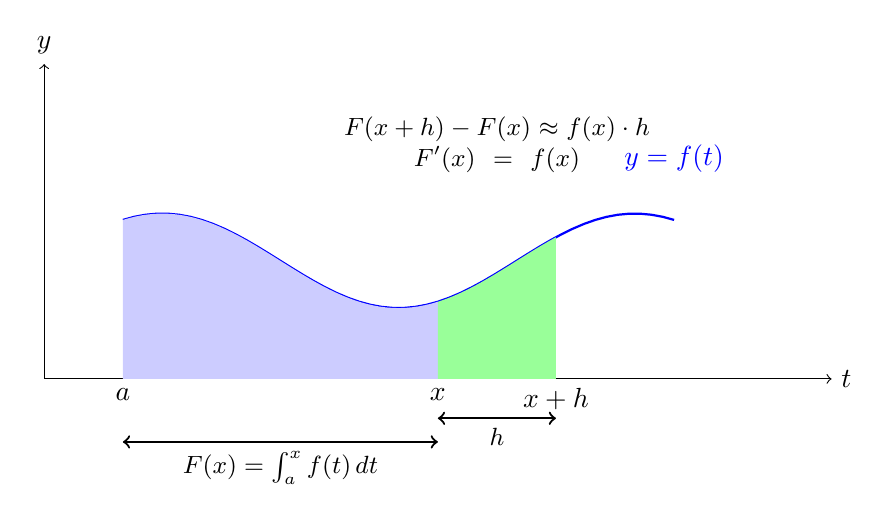
\begin{tikzpicture}[scale=1.0]
    \draw[->] (0, 0) -- (10, 0) node[right] {$t$};
    \draw[->] (0, 0) -- (0, 4) node[above] {$y$};
    
    % Function f(t)
    \draw[thick, blue, domain=1:8, samples=50] plot (\x, {1.5 + 0.6*sin(60*\x)});
    \node[above, blue] at (8, 2.5) {$y = f(t)$};
    
    % Shaded area from a to x
    \fill[blue!20, domain=1:5, samples=50] (1, 0) -- plot (\x, {1.5 + 0.6*sin(60*\x)}) -- (5, 0) -- cycle;
    
    % Points
    \node[below] at (1, 0) {$a$};
    \node[below] at (5, 0) {$x$};
    \node[below] at (6.5, 0) {$x+h$};
    
    % Extra area from x to x+h
    \fill[green!40, domain=5:6.5, samples=50] (5, 0) -- plot (\x, {1.5 + 0.6*sin(60*\x)}) -- (6.5, 0) -- cycle;
    
    % Labels
    \draw[<->, thick] (1, -0.8) -- (5, -0.8);
    \node[below, font=\small] at (3, -0.8) {$F(x) = \int_a^x f(t) \, dt$};
    
    \draw[<->, thick] (5, -0.5) -- (6.5, -0.5);
    \node[below, font=\small] at (5.75, -0.5) {$h$};
    
    \node[above, font=\small, text width=4cm, align=center] at (5.75, 2.5) {
        $F(x+h) - F(x) \approx f(x) \cdot h$ \\
        $\implies F'(x) = f(x)$
    };
\end{tikzpicture}
\end{center}

\begin{theorem}[Fundamental Theorem of Calculus, Part 2]\index{fundamental theorem of calculus!part 2}\index{FTC!part 2}
Let $f: [a, b] \to \mathbb{R}$ be continuous, and let $F$ be \textit{any} antiderivative of $f$ (i.e., $F'(x) = f(x)$).

Then:
\[\int_a^b f(x) \, dx = F(b) - F(a)\]

\textbf{Notation}: We write $F(b) - F(a) = \left[F(x)\right]_a^b$ or $F(x) \big|_a^b$.
\end{theorem}

\begin{proof}
By Part 1, we know that $G(x) = \int_a^x f(t) \, dt$ is an antiderivative of $f$.

Since $F$ is also an antiderivative of $f$, we have $F'(x) = G'(x) = f(x)$ for all $x \in (a, b)$.

By the theorem from Chapter 12 (antiderivatives differ by a constant), there exists $C$ such that:
\[F(x) = G(x) + C\]

Evaluating at $x = a$:
\[F(a) = G(a) + C = \int_a^a f(t) \, dt + C = 0 + C = C\]

Therefore $C = F(a)$, so $F(x) = G(x) + F(a)$.

Evaluating at $x = b$:
\[F(b) = G(b) + F(a) = \int_a^b f(t) \, dt + F(a)\]

Rearranging:
\[\int_a^b f(t) \, dt = F(b) - F(a)\]
$\blacksquare$
\end{proof}

\begin{keyidea}
\textbf{The Fundamental Theorem says}:

To compute $\int_a^b f(x) \, dx$, you don't need to compute limits of Riemann sums!

Instead:
\begin{enumerate}
    \item Find \textit{any} antiderivative $F$ of $f$ (i.e., $F' = f$)
    \item Evaluate $F(b) - F(a)$
\end{enumerate}

This transforms integration into antidifferentiation---a much easier problem.
\end{keyidea}

\begin{example}[Using FTC Part 2]
Compute $\int_0^2 x^2 \, dx$.

\textbf{Solution}: We need an antiderivative of $f(x) = x^2$.

Since $\frac{d}{dx}\left(\frac{x^3}{3}\right) = x^2$, we can take $F(x) = \frac{x^3}{3}$.

By FTC Part 2:
\[\int_0^2 x^2 \, dx = \left[\frac{x^3}{3}\right]_0^2 = \frac{8}{3} - \frac{0}{3} = \frac{8}{3}\]

$\blacksquare$

\textbf{Geometric verification}: The area under $y = x^2$ from $0$ to $2$ is indeed $\frac{8}{3}$ (can be verified by Riemann sums).
\end{example}

\begin{example}[Signed Areas]
Compute $\int_{-1}^1 x \, dx$.

\textbf{Solution}: $F(x) = \frac{x^2}{2}$ is an antiderivative of $x$.

\[\int_{-1}^1 x \, dx = \left[\frac{x^2}{2}\right]_{-1}^1 = \frac{1}{2} - \frac{1}{2} = 0\]

\textbf{Interpretation}: The area above the $x$-axis (for $x > 0$) exactly cancels the area below (for $x < 0$).

Integrals compute \textbf{signed area}, not total area. $\blacksquare$
\end{example}

\section{Integration Techniques}

\begin{theorem}[Substitution Rule]\index{substitution rule}\index{integration!substitution}\index{u-substitution}
Let $g: [a, b] \to \mathbb{R}$ be continuously differentiable, and let $f$ be continuous on the range of $g$.

Then:
\[\int_a^b f(g(x)) g'(x) \, dx = \int_{g(a)}^{g(b)} f(u) \, du\]

\textbf{Mnemonic}: Set $u = g(x)$, so $du = g'(x) \, dx$. Then ``substitute''.
\end{theorem}

\begin{proof}
Let $F$ be an antiderivative of $f$, so $F' = f$.

By the chain rule:
\[\frac{d}{dx}[F(g(x))] = F'(g(x)) \cdot g'(x) = f(g(x)) \cdot g'(x)\]

Therefore $F(g(x))$ is an antiderivative of $f(g(x)) g'(x)$.

By FTC Part 2:
\[\int_a^b f(g(x)) g'(x) \, dx = [F(g(x))]_a^b = F(g(b)) - F(g(a))\]

But also:
\[\int_{g(a)}^{g(b)} f(u) \, du = [F(u)]_{g(a)}^{g(b)} = F(g(b)) - F(g(a))\]

Therefore the two integrals are equal. $\blacksquare$
\end{proof}

\begin{example}[Substitution]
Compute $\int_0^1 2x e^{x^2} \, dx$.

\textbf{Solution}: Let $u = x^2$, so $du = 2x \, dx$.

When $x = 0$: $u = 0$. When $x = 1$: $u = 1$.

Therefore:
\[\int_0^1 2x e^{x^2} \, dx = \int_0^1 e^u \, du = [e^u]_0^1 = e - 1\]
$\blacksquare$
\end{example}

\begin{theorem}[Integration by Parts]\index{integration by parts}\index{integration!by parts}
If $u$ and $v$ are continuously differentiable on $[a, b]$, then:
\[\int_a^b u(x) v'(x) \, dx = [u(x)v(x)]_a^b - \int_a^b u'(x) v(x) \, dx\]

\textbf{Mnemonic}: $\int u \, dv = uv - \int v \, du$.
\end{theorem}

\begin{proof}
By the product rule:
\[\frac{d}{dx}[u(x)v(x)] = u'(x)v(x) + u(x)v'(x)\]

Rearranging:
\[u(x)v'(x) = \frac{d}{dx}[u(x)v(x)] - u'(x)v(x)\]

Integrating both sides from $a$ to $b$:
\[\int_a^b u(x) v'(x) \, dx = [u(x)v(x)]_a^b - \int_a^b u'(x) v(x) \, dx\]
$\blacksquare$
\end{proof}

\begin{example}[Integration by Parts]
Compute $\int_0^1 x e^x \, dx$.

\textbf{Solution}: Let $u = x$ (so $u' = 1$) and $v' = e^x$ (so $v = e^x$).

By integration by parts:
\begin{align*}
\int_0^1 x e^x \, dx &= [x e^x]_0^1 - \int_0^1 e^x \, dx \\
&= (1 \cdot e) - (0 \cdot 1) - [e^x]_0^1 \\
&= e - (e - 1) \\
&= 1
\end{align*}
$\blacksquare$
\end{example}

\section{Applications of Integration}

\begin{example}[Area Between Curves]
Find the area between $y = x^2$ and $y = x$ from $x = 0$ to $x = 1$.

\textbf{Solution}: The curves intersect at $x = 0$ and $x = 1$.

For $0 \leq x \leq 1$, we have $x \geq x^2$ (since $x - x^2 = x(1-x) \geq 0$).

Area between curves:
\begin{align*}
A &= \int_0^1 (x - x^2) \, dx \\
&= \left[\frac{x^2}{2} - \frac{x^3}{3}\right]_0^1 \\
&= \frac{1}{2} - \frac{1}{3} \\
&= \frac{1}{6}
\end{align*}
$\blacksquare$
\end{example}

\begin{center}
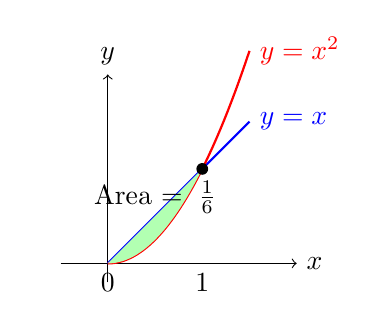
\begin{tikzpicture}[scale=1.2]
    \draw[->] (-0.5, 0) -- (2, 0) node[right] {$x$};
    \draw[->] (0, -0.2) -- (0, 2) node[above] {$y$};
    
    % Curves
    \draw[thick, blue, domain=0:1.5, samples=50] plot (\x, \x) node[right] {$y = x$};
    \draw[thick, red, domain=0:1.5, samples=50] plot (\x, {\x*\x}) node[right] {$y = x^2$};
    
    % Shaded area
    \fill[green!30, domain=0:1, samples=50] plot (\x, \x) -- plot[domain=1:0] (\x, {\x*\x}) -- cycle;
    
    % Labels
    \node[below] at (0, 0) {$0$};
    \node[below] at (1, 0) {$1$};
    \node[circle, fill=black, inner sep=1.5pt] at (1, 1) {};
    
    \node[text width=3cm, align=center] at (0.5, 0.7) {Area $= \frac{1}{6}$};
\end{tikzpicture}
\end{center}

\begin{example}[Arc Length]
The \textbf{arc length} of a curve $y = f(x)$ from $x = a$ to $x = b$ is:
\[L = \int_a^b \sqrt{1 + [f'(x)]^2} \, dx\]

\textbf{Derivation}: An infinitesimal segment has length:
\[ds = \sqrt{dx^2 + dy^2} = \sqrt{1 + \left(\frac{dy}{dx}\right)^2} dx = \sqrt{1 + [f'(x)]^2} \, dx\]

Integrating gives total arc length.

\textbf{Example}: Arc length of $y = x^{3/2}$ from $x = 0$ to $x = 1$:
\[L = \int_0^1 \sqrt{1 + \left(\frac{3}{2}x^{1/2}\right)^2} \, dx = \int_0^1 \sqrt{1 + \frac{9x}{4}} \, dx\]

(This can be computed using substitution $u = 1 + \frac{9x}{4}$.)
\end{example}

\begin{example}[Volume of Revolution]
Rotating $y = f(x)$ around the $x$-axis from $x = a$ to $x = b$ creates a solid with volume:
\[V = \pi \int_a^b [f(x)]^2 \, dx\]

\textbf{Derivation}: A thin disk at position $x$ has:
\begin{itemize}
    \item Radius: $r = f(x)$
    \item Thickness: $dx$
    \item Volume: $\pi r^2 dx = \pi [f(x)]^2 \, dx$
\end{itemize}

Integrating sums all disks.

\textbf{Example}: Volume of sphere of radius $R$:

Rotate $y = \sqrt{R^2 - x^2}$ (upper semicircle) around $x$-axis from $x = -R$ to $x = R$:
\begin{align*}
V &= \pi \int_{-R}^R (R^2 - x^2) \, dx \\
&= \pi \left[R^2 x - \frac{x^3}{3}\right]_{-R}^R \\
&= \pi \left[\left(R^3 - \frac{R^3}{3}\right) - \left(-R^3 + \frac{R^3}{3}\right)\right] \\
&= \pi \cdot \frac{4R^3}{3} = \frac{4\pi R^3}{3}
\end{align*}

The classical formula! $\checkmark$
\end{example}

\begin{center}
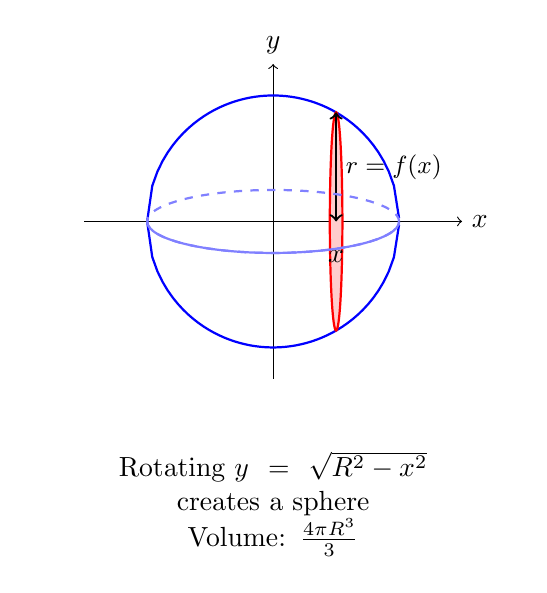
\begin{tikzpicture}[scale=0.8]
    % Revolution of curve
    \draw[->] (-3, 0) -- (3, 0) node[right] {$x$};
    \draw[->] (0, -2.5) -- (0, 2.5) node[above] {$y$};
    
    % Upper curve
    \draw[thick, blue, domain=-2:2, samples=50] plot (\x, {sqrt(4 - \x*\x)});
    \draw[thick, blue, domain=-2:2, samples=50] plot (\x, {-sqrt(4 - \x*\x)});
    
    % Disk at x
    \draw[thick, red, fill=red!20] (1, 0) ellipse (0.1 and 1.732);
    \node[below] at (1, -0.3) {$x$};
    \draw[<->, thick] (1, 0) -- (1, 1.732);
    \node[right, font=\small] at (1, 0.866) {$r = f(x)$};
    
    % 3D effect
    \draw[thick, blue!50, dashed] (2, 0) arc (0:180:2 and 0.5);
    \draw[thick, blue!50] (2, 0) arc (0:-180:2 and 0.5);
    \draw[thick, blue!50, dashed] (-2, 0) arc (180:360:2 and 0.5);
    
    \node[below, text width=6cm, align=center] at (0, -3.5) {
        Rotating $y = \sqrt{R^2 - x^2}$ creates a sphere \\
        Volume: $\frac{4\pi R^3}{3}$
    };
\end{tikzpicture}
\end{center}

\section{Improper Integrals}

\begin{definition}[Improper Integrals]
If $f$ is continuous on $[a, \infty)$, we define:
\[\int_a^\infty f(x) \, dx = \lim_{t \to \infty} \int_a^t f(x) \, dx\]
provided the limit exists.

Similarly, if $f$ has a vertical asymptote at $x = b$, we define:
\[\int_a^b f(x) \, dx = \lim_{t \to b^-} \int_a^t f(x) \, dx\]

If the limit exists (and is finite), the improper integral \textbf{converges}. Otherwise it \textbf{diverges}.
\end{definition}

\begin{example}[Convergent Improper Integral]
Compute $\int_1^\infty \frac{1}{x^2} \, dx$.

\textbf{Solution}:
\begin{align*}
\int_1^\infty \frac{1}{x^2} \, dx &= \lim_{t \to \infty} \int_1^t \frac{1}{x^2} \, dx \\
&= \lim_{t \to \infty} \left[-\frac{1}{x}\right]_1^t \\
&= \lim_{t \to \infty} \left(-\frac{1}{t} + 1\right) \\
&= 0 + 1 = 1
\end{align*}

Therefore $\int_1^\infty \frac{1}{x^2} \, dx = 1$ (converges). $\blacksquare$
\end{example}

\begin{example}[Divergent Improper Integral]
Compute $\int_1^\infty \frac{1}{x} \, dx$.

\textbf{Solution}:
\begin{align*}
\int_1^\infty \frac{1}{x} \, dx &= \lim_{t \to \infty} \int_1^t \frac{1}{x} \, dx \\
&= \lim_{t \to \infty} [\ln x]_1^t \\
&= \lim_{t \to \infty} (\ln t - \ln 1) \\
&= \lim_{t \to \infty} \ln t = \infty
\end{align*}

Therefore $\int_1^\infty \frac{1}{x} \, dx$ diverges. $\blacksquare$

\textbf{Moral}: $\int_1^\infty \frac{1}{x^p} \, dx$ converges if and only if $p > 1$.
\end{example}

\section{Looking Forward: Complex Numbers and Beyond}

\begin{intuition}
With integration, we've completed the core of \textbf{single-variable calculus}:
\begin{itemize}
    \item Limits and continuity
    \item Derivatives and rates of change
    \item Integrals and accumulation
    \item The Fundamental Theorem connecting them
\end{itemize}

\textbf{Next steps in the compendium}:
\begin{enumerate}
    \item \textbf{Complex numbers}: Extending $\mathbb{R}$ to $\mathbb{C}$, solving $x^2 + 1 = 0$
    \item \textbf{Abstract algebra}: Groups, rings, fields---the structure behind arithmetic
    \item \textbf{Linear algebra}: Vector spaces, matrices, linear transformations
    \item \textbf{Topology}: Generalizing continuity beyond $\mathbb{R}$
    \item \textbf{Multivariable calculus}: Derivatives and integrals in $\mathbb{R}^n$
\end{enumerate}

Each builds on the foundations we've laid.
\end{intuition}

\begin{center}
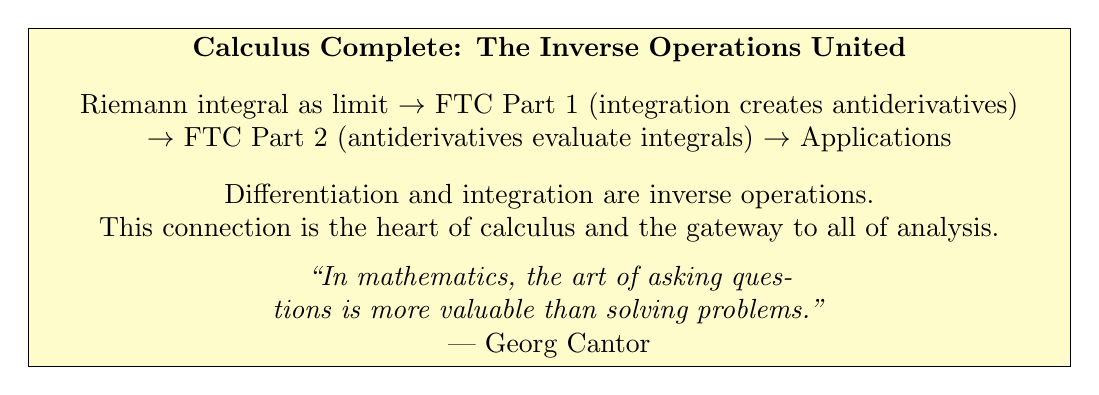
\begin{tikzpicture}[scale=1.0]
    \node[rectangle, draw, fill=yellow!20, text width=13cm, align=center] at (6.5, 0) {
    \textbf{Calculus Complete: The Inverse Operations United} \\[0.3cm]
    Riemann integral as limit $\to$ FTC Part 1 (integration creates antiderivatives) \\
    $\to$ FTC Part 2 (antiderivatives evaluate integrals) $\to$ Applications \\[0.3cm]
    Differentiation and integration are inverse operations. \\
    This connection is the heart of calculus and the gateway to all of analysis. \\[0.2cm]
    \textit{``In mathematics, the art of asking questions is more valuable than solving problems.''} \\
    --- Georg Cantor
    };
\end{tikzpicture}
\end{center}
